\subsection{Aplicación}

\subsubsection{Comportamiento de Aplicación}
El punto de vista Comportamiento de la aplicación describe el comportamiento interno de una aplicación.\\

Se puede ver en el caso de estudio, los diferentes componentes involucrados en el comportamiento y funcionalidad de la aplicación, se tiene en cuanta las visualización de la parte comercial de los músicos, su contratación, su pago, el sistema de recomendación, ...
\paragraph{Modelo}
\begin{figure}[h!]
	\centering
	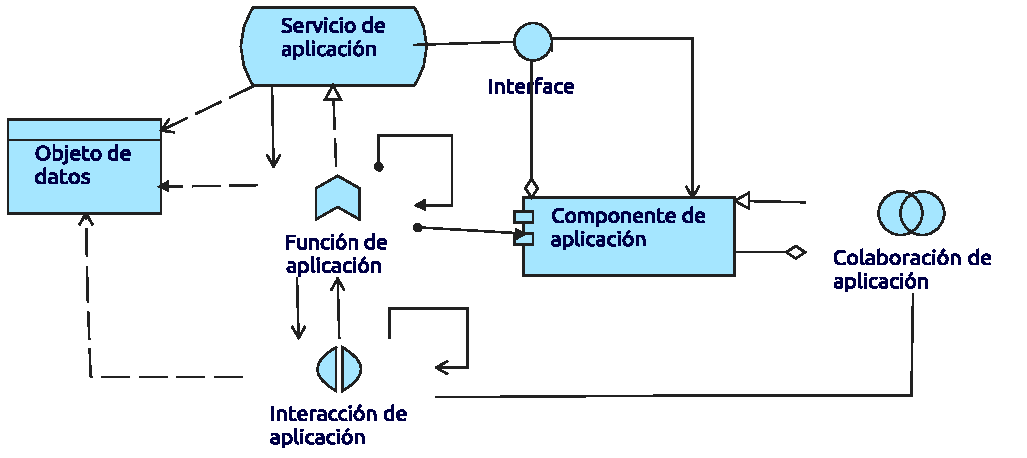
\includegraphics[width=0.8\linewidth]{Desarrollo/ArquitecturaEmpresarial/Aplicacion/imgs/ComportamientoMetamodelo.pdf}
	\caption{Modelo: Comportamiento de Aplicación}
\end{figure}
\newpage
\paragraph{Caso de Estudio}

\begin{figure}[h!]
	\centering
	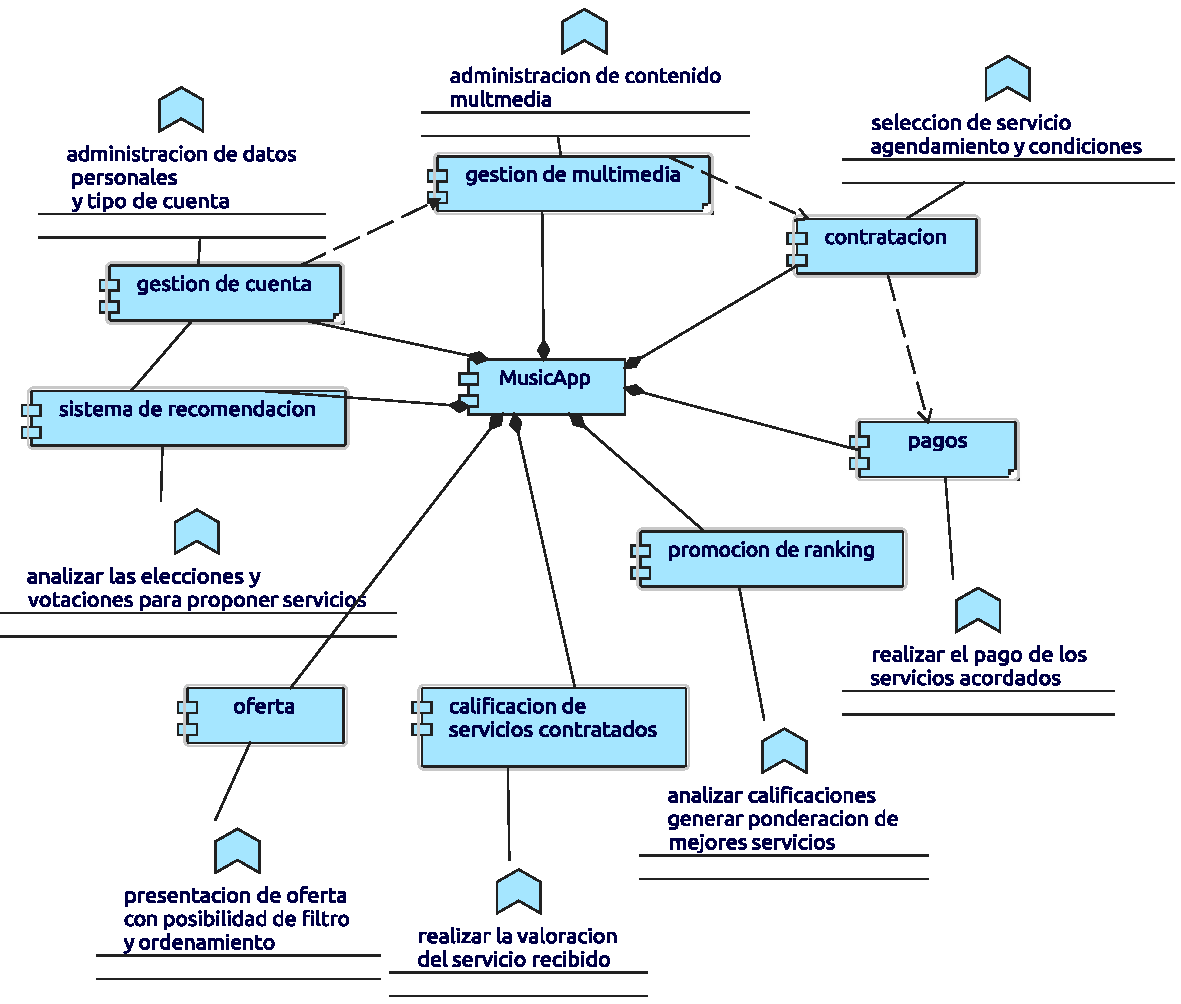
\includegraphics[width=\linewidth]{Desarrollo/ArquitecturaEmpresarial/Aplicacion/imgs/Comportamiento.pdf}
	\caption{Caso de estudio:  Comportamiento de Aplicación}
	\label{fig:comportamiento}
\end{figure}

\newpage

\subsubsection{Cooperación de Aplicación}
El punto de vista de la Cooperación en la Aplicación describe las relaciones entre los componentes de las aplicaciones en términos de los flujos de información entre ellos, o en términos de los servicios que ofrecen y utilizan. \\

En el caso de estudio, se  crear una visión general del panorama de aplicaciones de una organización. se divide en dos, la parte del front y el back, la primera hacer referencia lo que esta en contacto directo con los principales actores y en el back, hace referencia a todos los proceso que se hacen sin incolucrar directamente los actores.
\paragraph{Modelo}
\begin{figure}[h!]
	\centering
	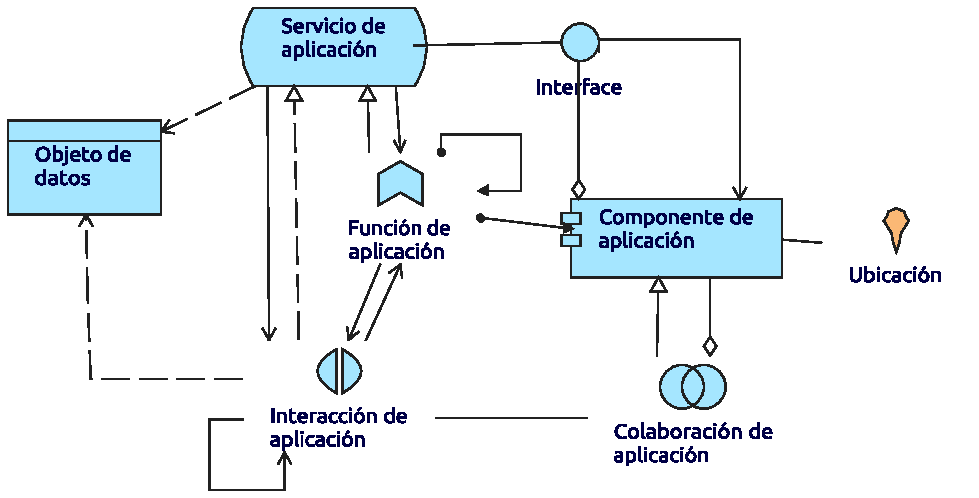
\includegraphics[width=\linewidth]{Desarrollo/ArquitecturaEmpresarial/Aplicacion/imgs/CooperacionMetamodelo.pdf}
	\caption{Modelo: Cooperación de Aplicación}
\end{figure}
\newpage
\paragraph{Caso de Estudio}

\begin{figure}[h!]
	\centering
	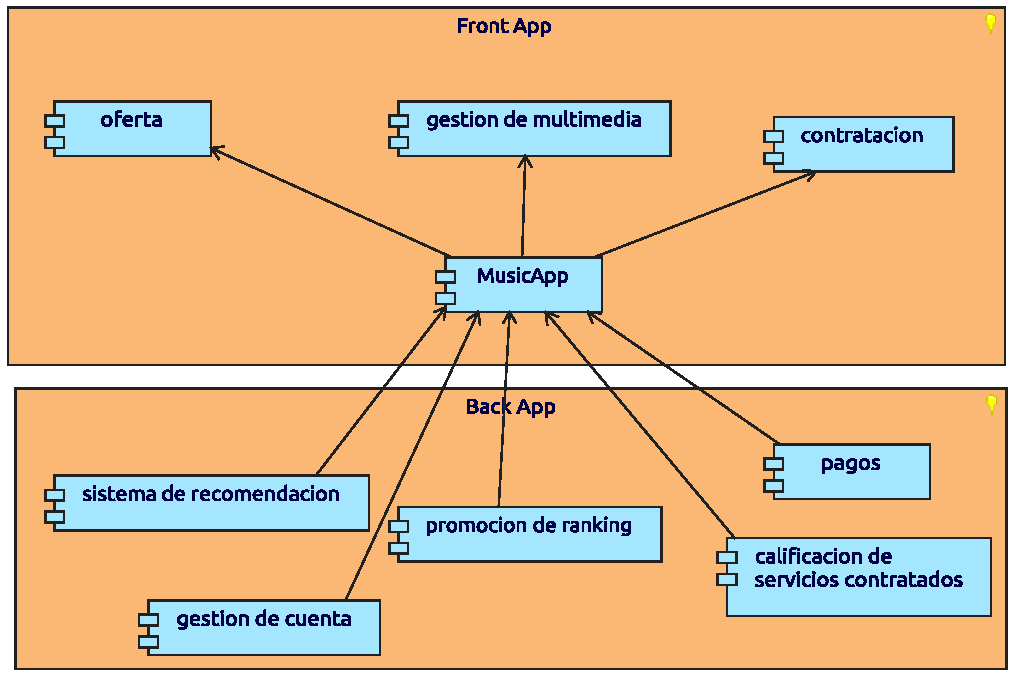
\includegraphics[width=\linewidth]{Desarrollo/ArquitecturaEmpresarial/Aplicacion/imgs/Cooperacion.pdf}
	\caption{Caso de estudio: Cooperación de Aplicación }
\end{figure}

\newpage

\subsubsection{Estructura de Aplicación}
El punto de vista de la Estructura de la aplicación muestra la estructura de una o más aplicaciones o componentes. \vspace{\baselineskip}

Para el caso de estudio, se representan las principales interfaces de la aplicación y sus respectivos componentes, las principales interfaces son: Publicación, Multimedia, Contratación, Recaudo, Puntuación, Promoción, Cuenta y Recomendación. \vspace{\baselineskip}

Y así con la Figura \ref{fig:comportamiento} se puede combinar para genera el código presentado a continuación.
\paragraph{Modelo}
\begin{figure}[h!]
	\centering
	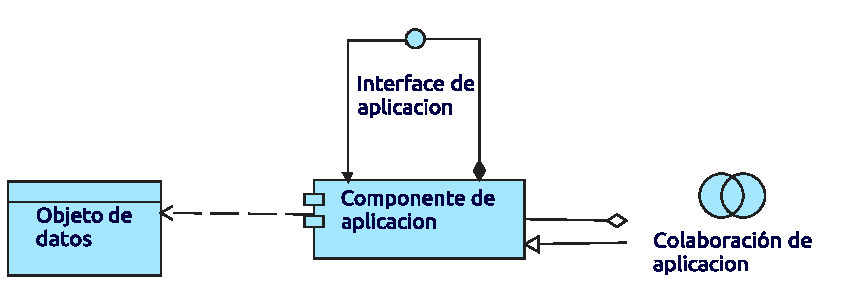
\includegraphics[width=\linewidth]{Desarrollo/ArquitecturaEmpresarial/Aplicacion/imgs/estructuraMetamodelo.pdf}
	\caption{Modelo: Estructura de Aplicación}
\end{figure}
\newpage
\paragraph{Caso de Estudio}

\begin{figure}[h!]
	\centering
	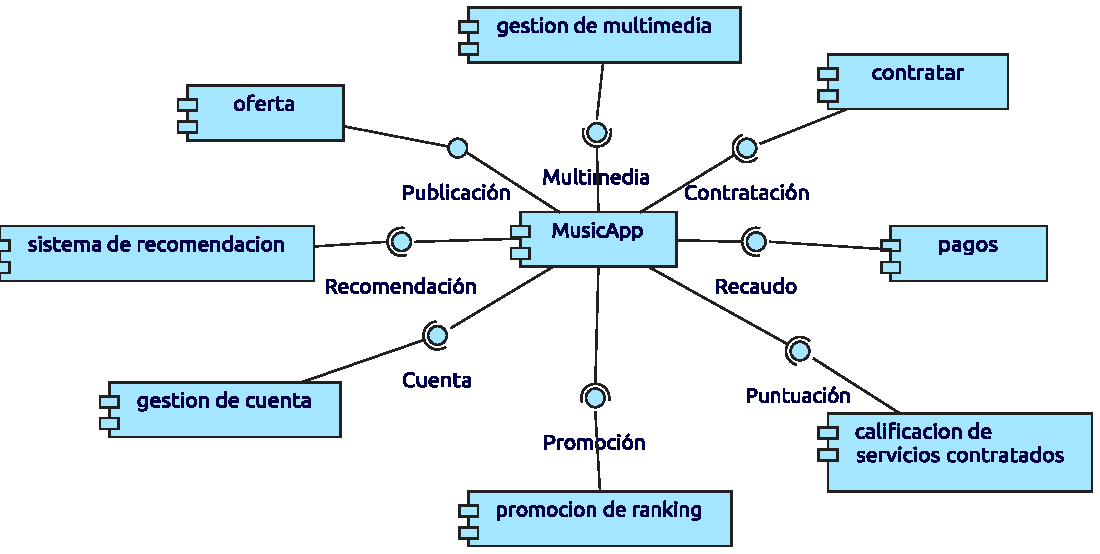
\includegraphics[width=\linewidth]{Desarrollo/ArquitecturaEmpresarial/Aplicacion/imgs/estructura.pdf}
	\caption{Caso de estudio: Estructura de Aplicación }
\end{figure}


\paragraph{Código}

\lstinputlisting[language=Java]{Desarrollo/ArquitecturaEmpresarial/Aplicacion/fuentes/IContratacion.java}
\lstinputlisting[language=Java]{Desarrollo/ArquitecturaEmpresarial/Aplicacion/fuentes/ICuenta.java}
\lstinputlisting[language=Java]{Desarrollo/ArquitecturaEmpresarial/Aplicacion/fuentes/IMultimedia.java}
\lstinputlisting[language=Java]{Desarrollo/ArquitecturaEmpresarial/Aplicacion/fuentes/IPromocion.java}
\lstinputlisting[language=Java]{Desarrollo/ArquitecturaEmpresarial/Aplicacion/fuentes/IPublicacion.java}
\lstinputlisting[language=Java]{Desarrollo/ArquitecturaEmpresarial/Aplicacion/fuentes/IPuntuacion.java}
\lstinputlisting[language=Java]{Desarrollo/ArquitecturaEmpresarial/Aplicacion/fuentes/IRecaudo.java}
\lstinputlisting[language=Java]{Desarrollo/ArquitecturaEmpresarial/Aplicacion/fuentes/IRecomendacion.java}
\newpage

\subsubsection{Uso de Aplicación}

El punto de vista de Uso de la aplicación describe cómo se usan las aplicaciones para admitir uno o más procesos de negocios, y cómo las usan otras aplicaciones. \vspace{\baselineskip}

El el caso de estudio, se puede ver el proceso de contratación, y sus procesos asociados a este, y su interacción entre lo servicios y los componentes que las integran para lograr el proceso deseado.
\paragraph{Modelo}
\begin{figure}[h!]
	\centering
	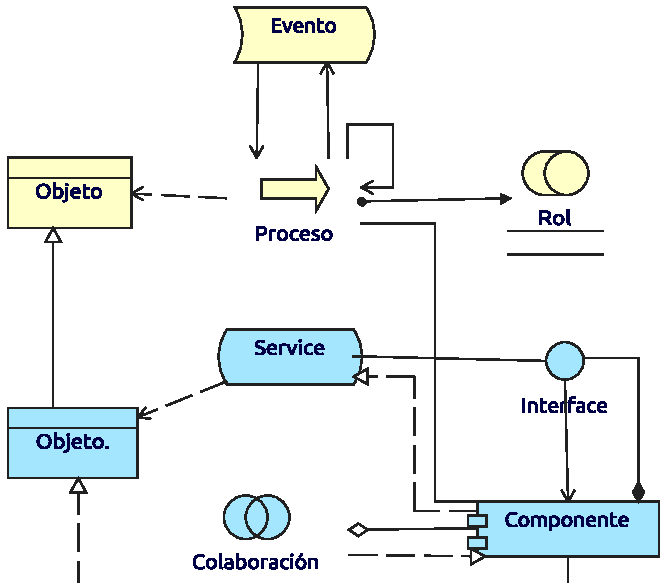
\includegraphics[width=0.9\linewidth]{Desarrollo/ArquitecturaEmpresarial/Aplicacion/imgs/uso.pdf}
	\caption{Modelo: Uso de Aplicación}
\end{figure}
\newpage
\paragraph{Caso de Estudio}

\begin{figure}[h!]
	\centering
	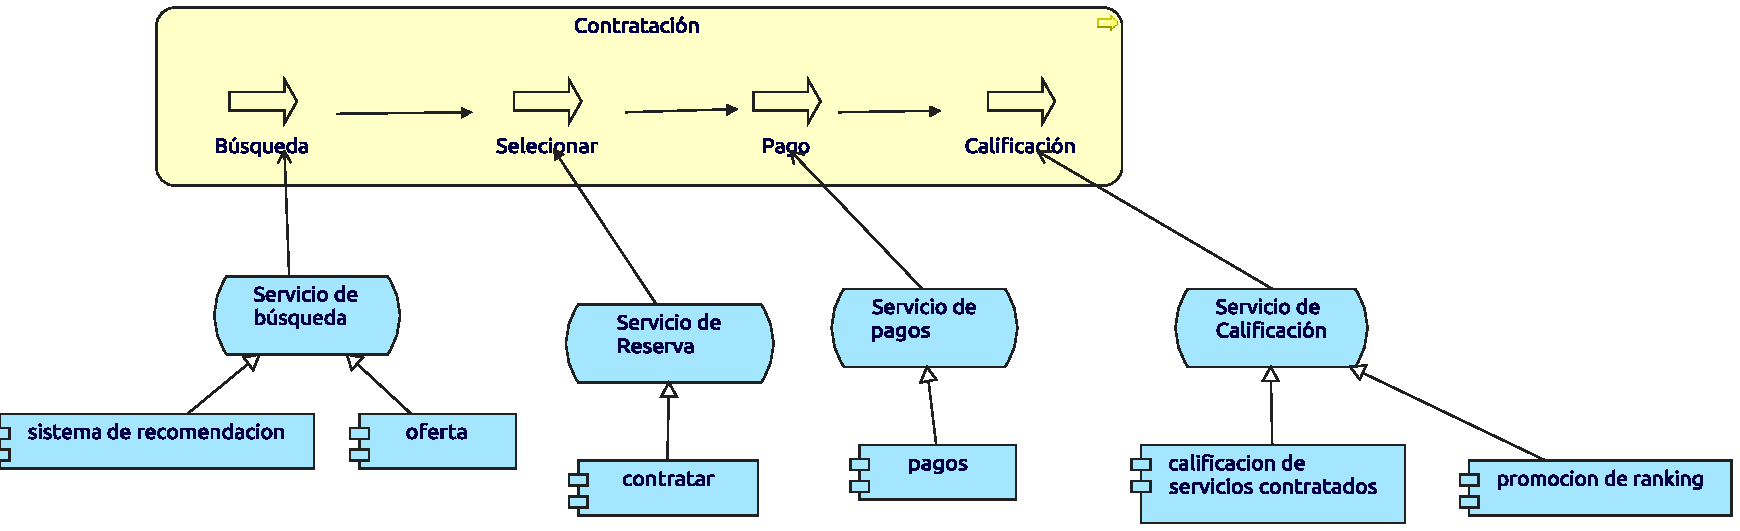
\includegraphics[width=\linewidth]{Desarrollo/ArquitecturaEmpresarial/Aplicacion/imgs/usoMetamodelo.pdf}
	\caption{Caso de estudio: Uso de Aplicación}
\end{figure}